\documentclass[12pt, en, oneside, openany]{mgr}
\usepackage[utf8]{inputenc}
\usepackage[T1]{fontenc}

%Additional
\usepackage[nottoc,notlot,notlof]{tocbibind} %Add bibliography to contents
\usepackage{hyperref} %Add links to contents
\hypersetup{colorlinks, citecolor=black, filecolor=black, linkcolor=black, urlcolor=black} %Links styling
\usepackage{indentfirst} %Indentation in first paragraphs

\usepackage{graphicx} %Enable include graphics
\graphicspath{ {./Graphics/} } %Path to graphics
\usepackage{float} %Parameter H in figure

\usepackage{subcaption} 

\usepackage{amssymb} %Math expressions
\usepackage{amsmath} %Math expressions
\usepackage{amsthm} %Math expressions

% Title page
\title{Badania metod zmiany obiektów na obrazach z wykorzystaniem technologii Deepfake}
\engtitle{Research on methods of changing objects in images using Deepfake technology}
\author{Michał Zendran}
\supervisor{Dr hab. inż. Andrzej Rusiecki}
\field{Computer Science}
\specialisation{Internet Engineering (INE)}

\begin{document}

\maketitle
\tableofcontents
\newpage
	
\chapter{Abstract}
Deepfake is a technique from image-to-image translation class of problems, designed to combine and overlay objects in images or videos creating deceptively realistic counterfeits. This paper analyzes and compares four leading methods used for deepfake generation: autoencoders, variational autoencoders,  variational autoencoders generative adversarial networks and cycle generative adversarial networks, in problem of face-to-face conversion. Due to the lack of numerical methods for deepfake comparison, all obtained results were assessed in a visual evaluation process. Variational autoencoders technique has proved to be the most efficient one in facial-deepfake generation problem. The worst results were obtained from CycleGAN method, which proved to be unfitted for geometric changes and shape transformations. It was concluded that VAE-GAN technique is the one with the greatest potential, as in case of feature maps with better quality, this approach could provide deceivingly resembling deepfakes.
\chapter{Introduction}
\section{Motivation}
Machine learning has found many, different applications in the field of image data processing and computer vision. From picture classification to image denoiseing and resolution enhancement, artificial neural networks has gained the opinion of exceptionally useful tool. But for some time, a new, controversial use-case has been getting more and more attention in both media and research circles. So-called "deepfake" technology has opened doors to many new possibilities of picture generation, but also raised many issues of moral and legal matters.\\

Deepfake is a technology from the field of machine learning designed to combine and overlay objects in images or videos creating deceptively realistic counterfeits. The name comes from combination of two terms: ``deep learning'' and ``fake'', and has its origins in a Reddit user named ``deepfakes''. Initially the term was associated only with face-swapping technology, but with time it was extended to all deep learning implementations of changing objects in images.\\

Deepfake technology has already found multiple applications such as changing seasons in the landscapes images, transforming horses into zebras or "repainting" images in styles of different artists. But the most controversial and impactful use-case so far is already mentioned face-swapping. In times of overwhelming amount of news it's getting harder and harder to filter out fake ones from valuable peaces of information. People generally tend not to check sources of information but rather blindly follow hot stories in social medias and television. Such environment combined with capabilities of deepfake gives possibilities of influencing elections by misrepresenting politicians in forged videos to defame or blackmail theme. Another popular use-case of described technology is creating erotic videos by replacing faces of porn actress with faces of well-known celebrities. This application might have less dangerous consequences than influencing world politics but may be hurtful to people that became objects of such act.\\

Although there are many malicious ways of using deepfake technology it might also be used for good reasons such as helping people to cope with the loss of the loved once or in entertainment filed by de-ageing actors to play younger-selves. Besides, to be able to detect and fight harmful applications of deepfake it might be vital to deeply understand algorithms  and techniques behind it. Therefore, conducting research on that part of machine learning field seems to have great meaning in incoming times.

\section{Objective and assumptions}
This project aims to implement and compare four different methods of changing objects in images with application of artificial neural networks. For sake of this research, human faces were chosen as an object of replacement, as it rises a complex issue of simultaneous color, texture and shape modification.\\

As there are no numerical methods of measuring the quality of images obtained from deepfake algorithms, the only way of appraising results of methods discussed in this research is visual evaluation. To be able to fairly rate each implemented technique, the same set of images will be used as a learning dataset for all cases. Therefor, effects of all approaches will be visually evaluated and compared with each other, which will result in the final assessment. This rating of methods is the expected outcome of the research.\\

There are two main factors that will be taken into a consideration during a results evaluation process. First of them is a resemblance of the faked image, to the appearance of the imitated person. The more striking similarity, the better. The other crucial aspect is preservation of original facial expression and pose, as the believable deepfake must capture the source material movements. Resultant of those two factors will be the main feature to be rated. It is assumed that neither of mentioned characteristics should outweigh the other one, but rather, the final effect should be well-balanced composition of both aspects.

\section{State of the art}
While there are many, great articles and papers that elaborately explain all mentioned approaches of generating deepfakes, no comparison of those methods were found. To be written ...



\section{Naming conventions and terminology}
Below, all abbreviations and naming conventions used in this research are listed and explained:

\begin{itemize}
\item Deepfake -- name of the deep learning technology of swapping objects in images or an end result generated witch such technology
\item ANN -- artificial neural network
\item CNN -- convolutional neural network
\item AE -- autoencoder 
\item VAE -- variational autoencoder
\item GAN -- generative adversarial network
\item VAE-GAN -- variational autoencoder-generative adversarial network 
\item Activation function -- transfer function
\item GPU -- graphics processing unit
\end{itemize}
\chapter{Theoretical background}
\section{Artificial neural network}
Explain what are ANN, its training and types like CNN

\section{Deepfake}
Maybe change this section name from deepfake to CNN and explain what is CNN instead of explaining it in previous section?
\chapter{Deepfake methods}
\section{Autoencoder}
\label{Autoencoder}
Autoencoders are the most basic approach to the problem of deepfake generation. In fact, all mentioned methods, except for CycleGAN, are just different variations of this idea. Autoencoder is a type of artificial neural network that learns to reproduce given input in an unsupervised manner. The goal is to train functions \(A: \mathbb{R}^n \to \mathbb{R}^p\) (encoder) and \(B: \mathbb{R}^p \to \mathbb{R}^n\) (decoder) to satisfy condition given in equation \ref{eq:autoencoder_condition} as described in \cite{autoencoders_bib},
%
\begin{equation}
\label{eq:autoencoder_condition}
arg \, min_{A,B} E[\Delta(x,B \circ A(x))]
\end{equation}
%
where \(E\) -- expectation over the distribution of \(x\) and \(\Delta\) -- reconstruction loss function, which measures the distance between given input and the output of the decoder. General idea of autoencoder model is illustrated in figure \ref{fig:autoencoder_general_idea}. Typically, architecture of autoencoder consists not only of input and output layers, as this would result in simple coping pixels from the input to the output of the network, but also contains single or multiple hidden layers in between, with the number of neurons lesser than the number of pixels in the input image. Such structure causes bottleneck effect and creates so-called compressed representation at the output of the encoder part, known also as ``feature map'' or in case of deepfake ``latent face''. Such compression causes feature map to preserve only information most relevant for later reconstruction and gets rid of unnecessary data.

\begin{figure}[H]
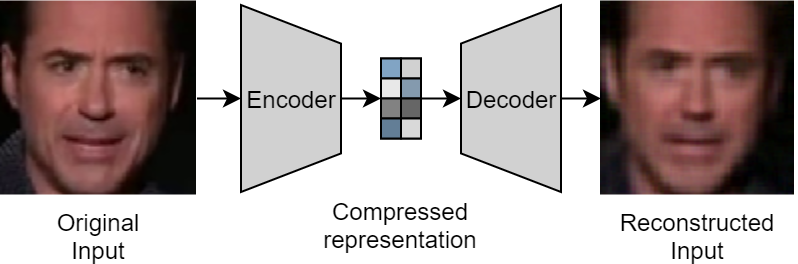
\includegraphics[width=12cm] {autoencoder_general_idea.png}
\centering
\caption{General idea of autoencoder}
\label{fig:autoencoder_general_idea}
\end{figure}

Generating deepfakes using autoencoders approach consists of three major steps. Described process is illustrated in figure \ref{fig:deepfake_steps}. Let us assume that \(X\) is a set of face images of person \(x\) and \(Y\) is a set of face images of person \(y\). Firstly, as shown in figure \ref{subfig:deepfake_steps_a}, an encoder is trained to produce feature maps for images of faces from both classes. Simultaneously, a corresponding decoder (further called decoder XY) is trained as a measure of encoder accuracy. Afterwards, two decoders (further called decoder X and decoder Y) are trained separately to reproduce original images from latent faces generated by pre-trained encoder, as presented in figure \ref{subfig:deepfake_steps_b}. Finally, decoders are switched to produce images from one class based on feature maps from the other class, which was illustrated in figure \ref{subfig:deepfake_steps_c}.

\begin{figure}[H]
\centering
\begin{subfigure}{12cm}
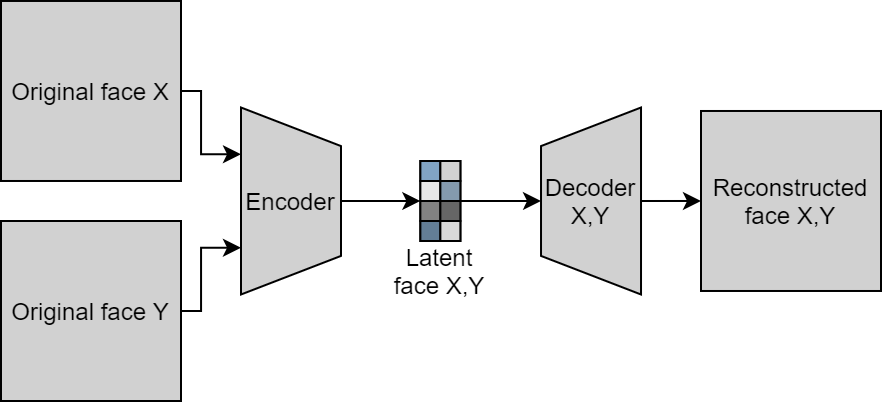
\includegraphics[width=\textwidth]{deepfake_idea_1.png}
\caption{Training autoencoder}
\label{subfig:deepfake_steps_a}
\end{subfigure}

\begin{subfigure}{12cm}
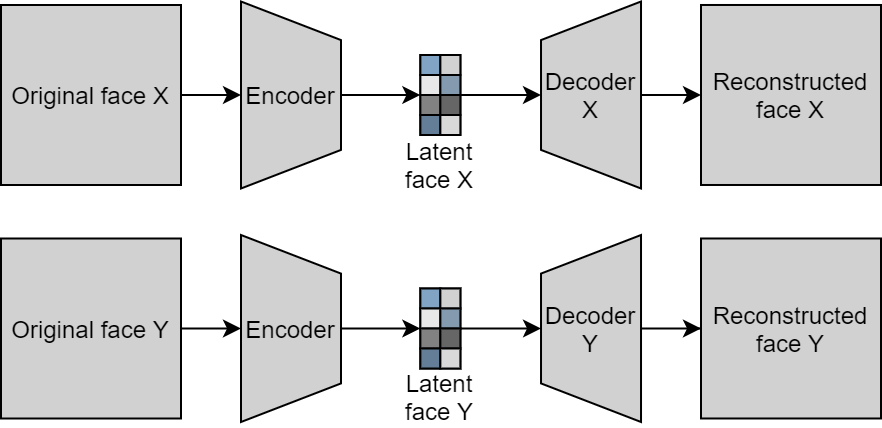
\includegraphics[width=\textwidth]{deepfake_idea_2.png}
\caption{Training decoders X and Y}
\label{subfig:deepfake_steps_b}
\end{subfigure}

\begin{subfigure}{12cm}
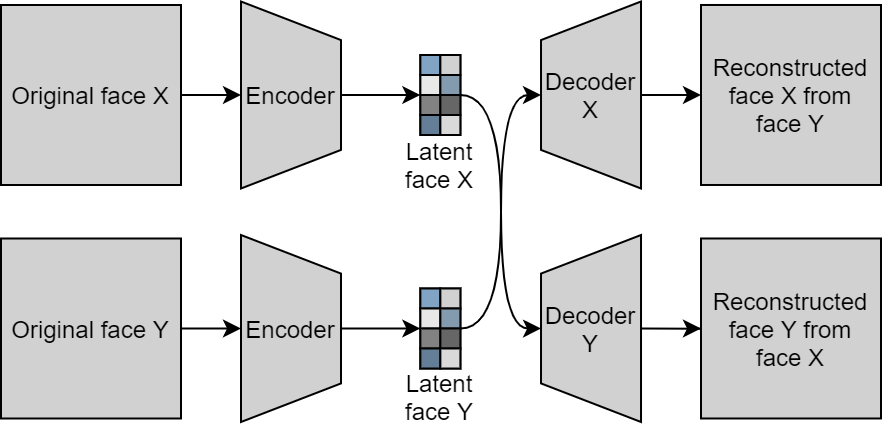
\includegraphics[width=\textwidth]{deepfake_idea_3.png}
\caption{Generating X from Y and Y from X}
\label{subfig:deepfake_steps_c}
\end{subfigure}

\caption{Three steps of generating deepfakes}
\label{fig:deepfake_steps}
\end{figure}

\newpage
\section{Variational autoencoder}
\label{Variational_autoencoder}
Unlike basic autoencoders, which purpose is to reproduce given input by ``memorizing'' it, variational autoencoders aim to produce latent vectors (feature maps) that follow a unit Gaussian distribution \cite{variational_bayes_bib}. Such modification allows to generate new images by sampling a latent vector from the unit Gaussian distribution and pass it as an input of the decoder network. The goal in VAE model training is to optimize the loss function given in equation \ref{eq:vae_loss} \cite{vae_loss_bib}. First component of this function is a reconstruction loss \(\mathcal{L}_{rec}\), which, by comparing pixels from image \(x\), encoded to a latent vector \(z = Encoder(x) \sim q(z|x)\), and reconstructed image \(\bar{x} = Decoder(z) \sim p(x|z)\), measures expected marginal log-likelihood of the observations in \(x\). Second component, so called Kullback–Leibler divergence \cite{kl_divergence_bib}, measures the extent to which one probability distribution differs from another. Applying KL divergence to VAE loss function allows to control distribution of the latent vector \(z\).
%
\begin{equation}
\label{eq:vae_loss}
\mathcal{L}_{vae} = \mathcal{L}_{rec} + \mathcal{L}_{kl}
\end{equation}
%
\begin{equation}
\label{eq:rec_loss}
\mathcal{L}_{rec} = -E_{q(z|x)}[\log{p(x|z)}]
\end{equation}
%
\begin{equation}
\label{eq:kl_loss}
\mathcal{L}_{kl} = D_{kl}(q(z|x)||p(z|x))
\end{equation}

Presence of KL divergence in VAE loss function generates problem with applying backpropagation to the encoder network, as decoder randomly samples from latent vector \(z\) and backpropagation cannot flow through random node as in figure \ref{subfig:before_reparameterization}. As a solution, a ``reparameterization trick'' is introduced \cite{reparameterization_trick_bib}. This method maps the output of an encoder to separate vectors, mean \(\mu\) and standard deviation \(\sigma\), instead of a z-dimensional latent vector. Such representation allows to calculate \(z\) in a following way:
%
\begin{equation}
\label{eq:rec_loss}
z = \mu + \sigma\epsilon
\end{equation}
%
where \(\epsilon\) is sampled from a multivariate standard normal distribution (\(Normal(0,1)\)) and therefore acts as a stochastic component. Such reparameterization allows to run backpropagation process as now latent vector is not purely random, but consists of deterministic and stochastic nodes as illustrated in figure \ref{subfig:after_reparameterization}.

\begin{figure}[H]
\centering
\begin{subfigure}{.5\textwidth}
  \centering
  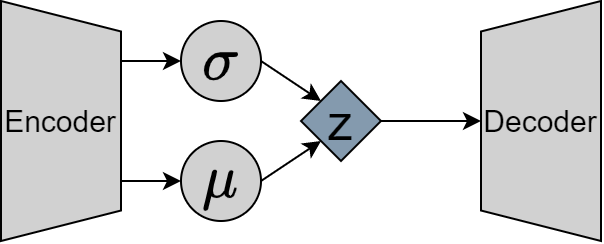
\includegraphics[width=0.9\linewidth]{before_reparameterization.png}
  \caption{Nodes before reparameterization}
  \label{subfig:before_reparameterization}
\end{subfigure}%
\begin{subfigure}{.5\textwidth}
  \centering
  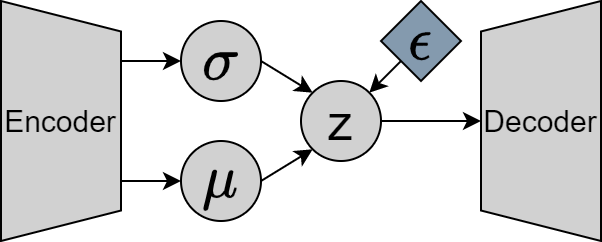
\includegraphics[width=0.9\linewidth]{after_reparameterization.png}
  \caption{Nodes after reparameterization}
  \label{subfig:after_reparameterization}
\end{subfigure}
\caption{Reparameterization trick}
\label{fig:reparameterization_trick}
\end{figure}

By applying reparameterization trick to equation \ref{eq:kl_loss}, Kullback–Leibler divergence takes following form \cite{kl_divergence_loss_bib}:
%
\begin{equation}
\label{eq:final_kl_loss}
\mathcal{L}_{kl} = -\frac{1}{2}\sum_{i=0}^{z}(1 + \log(\sigma_i^2) - \mu_i^2 -\sigma_i^2)
\end{equation}

Generating deepfakes using variational autoencoders approach is based on the same algorithm as autoencoders approach illustrated in figure \ref{fig:deepfake_steps}. The only difference between those two methods is the way the latent face (latent vector) is obtained.

\section{VAE-GAN}
\label{VAE-GAN}
As the name suggests, variational autoencoder generative adversarial network is a combination of previously mentioned VAEs and GANs. By combining those two approaches it is possible to leverage learned representations to better measure similarities in data space \cite{autoencoding_beyond_pixels_bib}. General idea of this technique is similar to the one described in section \ref{Variational_autoencoder}, but instead of VAE's decoder, a GAN generator is used to decode feature maps, as illustrated in figure \ref{fig:vaegan_general_idea}.

\begin{figure}[H]
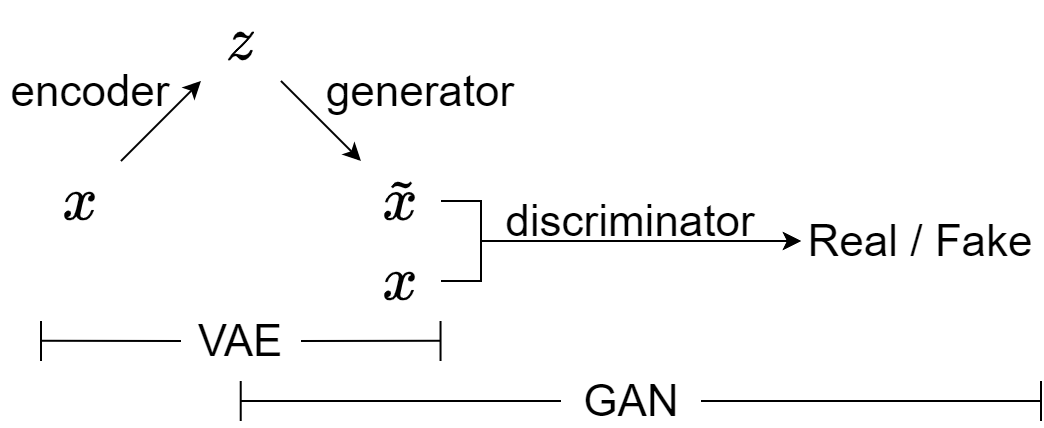
\includegraphics[width=9cm] {vaegan_general_idea.png}
\centering
\caption{General idea of VAE-GAN}
\label{fig:vaegan_general_idea}
\end{figure}

The whole potential of this method comes from the discriminator part. This network, during the training process, learns to distinguish real images (pictures before encoding) from generated ones. On the other side, generator network ``tries'' to deceive the discriminator by producing better and better fake images, improving the quality of final deepfakes. General idea of GAN training process is ilustrated in figure \ref{fig:gan_general_idea}. To train VAE-GAN model, three different loss functions, applied to corresponding networks, are required: encoder loss, generator loss and discriminator loss:
%
\begin{equation}
\label{eq:encoder_loss}
\mathcal{L}_{Enc} = -E_{q(z|x)}[\log{p(x|z)}] + D_{kl}(q(z|x)||p(z|x))
\end{equation}
%
\begin{equation}
\label{eq:generator_loss}
\mathcal{L}_{Gen} = -E_{q(z|x)}[\log{p(x|z)}] * \gamma - \log(Dis(X)) - \log(1 - Dis(\tilde{X}))
\end{equation}
%
\begin{equation}
\label{eq:discriminator_loss}
\mathcal{L}_{Dis} = \log(Dis(X)) + \log(1 - Dis(\tilde{X}))
\end{equation}
%
where \(\tilde{X}\) - fake image generated from encoded image \(X\), \(\gamma\) - weight factor to balance the loss function value. 

\begin{figure}[H]
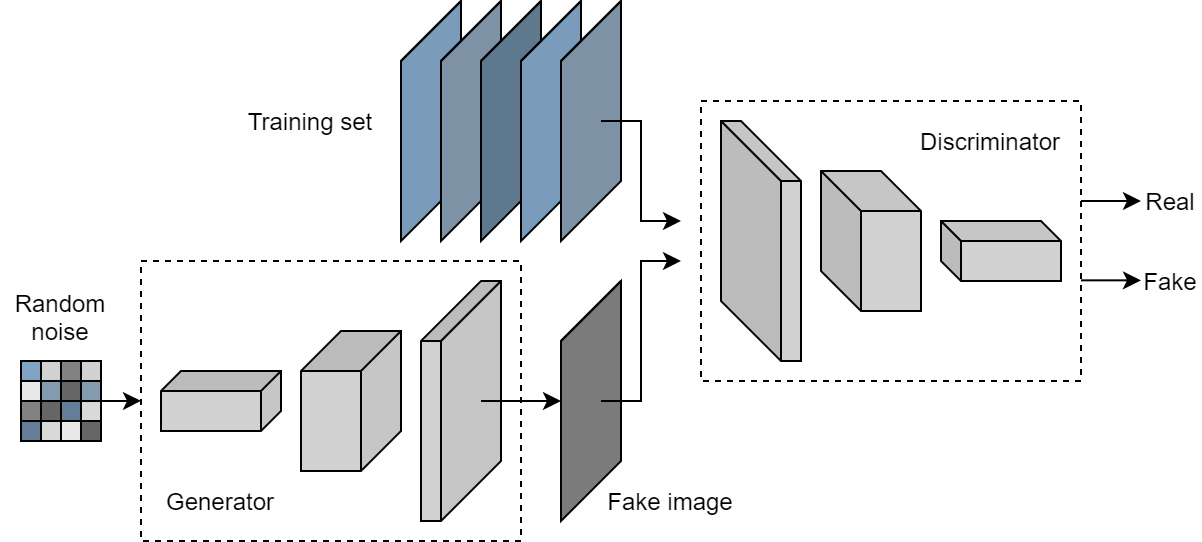
\includegraphics[width=14cm] {gan_general_idea.png}
\centering
\caption{General idea of GAN}
\label{fig:gan_general_idea}
\end{figure}

\section{CycleGAN}
CycleGAN is an approach to the image-to-image translation problems, based on deep learning techniques, which does not require a dataset of paired images. Typically, CycleGAN model's architecture consists of two GAN networks, where one generator (\(G:X \to Y\)) is responsible for generating images for one class, and the other (\(F:Y \to X\)) for generating images for the second one \cite{cycleGAN_4_bib}. The goal of the training process is given in the equation \ref{eq:cyclegan_condition1}, as described in \cite{cycleGAN_5_bib},
%
\begin{equation}
\label{eq:cyclegan_condition1}
G^*,F^* = arg \, \min_{G,F} \, \max_{D_X,D_Y} \mathcal{L}(G,F,D_X,D_Y)
\end{equation}
%
\begin{equation}
\label{eq:cyclegan_condition2}
\mathcal{L}(G,F,D_X,D_Y) = \mathcal{L}_{GAN}(G,D_Y,X,Y) + \mathcal{L}_{GAN}(F,D_X,Y,X) + \lambda\mathcal{L}_{cyc}(G,F)
\end{equation}
%
where \(X,Y\) -- image domains, \(D_Y\) -- discriminator for  the mapping function \(G\), \(D_X\) -- discriminator for  the mapping function \(Y\), \(\lambda\) -- weight factor to balance the loss function value.\\

General idea of CycleGAN is to have both generators \(G,F\) to convert images from one domain to another, in a GAN's manner, described in section \ref{VAE-GAN}. However, depending only on the GAN's adversarial loss alone do not ensure that images after conversion will maintain important features from its original class. To solve this problem, a cycle consistency loss is applied to the final loss function, as in equation \ref{eq:cyclegan_condition2}. It relies on the expectation, that image converted by both generators \(G,F\) from one domain to the other, and than back again, should look the same as at the beginning. General idea of this process is illustrated in the figure \ref{fig:cyclegan_general_idea}.\\

\begin{figure}[H]
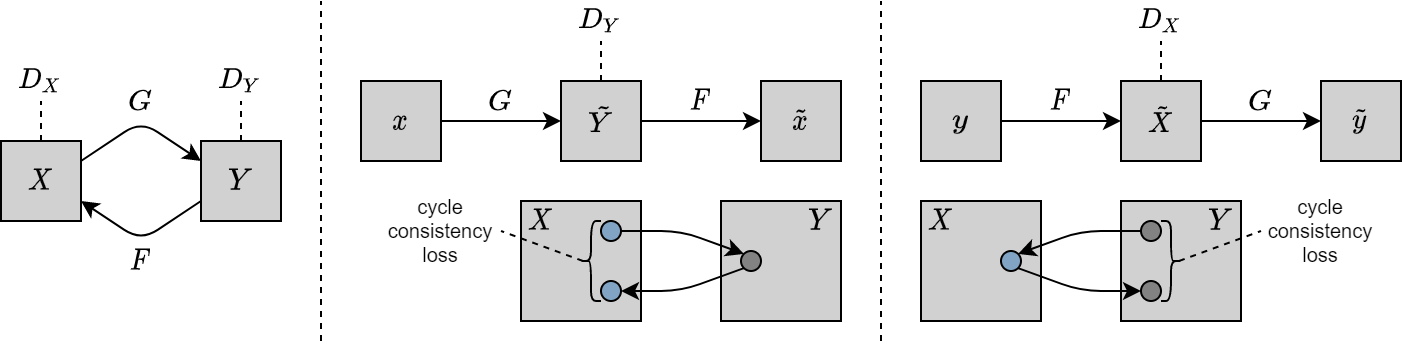
\includegraphics[width=\textwidth] {cyclegan_general_idea.png}
\centering
\caption{General idea of CycleGAN}
\label{fig:cyclegan_general_idea}
\end{figure}

CycleGAN networks have proven to be very efficient in many image-to-image translation problems. The most popular applications are:

\begin{itemize}
\item changing art styles in images of paintings
\item coloring black and white images
\item changing the season of the landscape in a photo
\item transforming horses into zebras
\item transforming apples into oranges
\end{itemize}
\chapter{Datasets}
\section{Dataset description}
Creating a high quality, well-balanced dataset is an essential step in the process of deepfake generation. Poorly prepared training set might cause that even great network architectures and state of the art algorithms will produce disappointing results. The most efficient approach to this problem ,in case of face-swapping technology, is obtaining images of targeted people from video recordings, which allows to produce great number of images that cover different facial expressions and head positions. There are several factors that should be taken into a consideration in order to construct proper dataset.\\

First of all, videos of people with at least slight resemblance should be chosen. The most important feature in this matter is skin tone but the more similar appearances, the more deceiving deepfake might be achieved. Another important factor is overall quality of source material. Videos with high resolution and large number of frames per second are best suited for this purpose, but also require more computational power and time to properly train necessary networks. Finally, after deconstruction of videos into single images, all set should be revised to remove pictures that depict faces which are blurry, deformed or in some way covered, for example by hand.\\

For sake of this research the ``VoxCeleb2'' dataset was used. As described in \cite{voxceleb2_bib}, VoxCeleb2 consists of over 1 million utterances of over 6000 celebrities derived from videos from YouTube platform. Source data is diversified in terms of recorded people's genders, ethnicities, ages and accents but also in terms of videos quality, lighting conditions, stability and lengths. Each recording has a resolution of 224 by 224 pixels and depicts closeup shot of a character's face and shoulders, which is close enough to clearly capture subtle facial expressions.

\section{Data pre-processing}
To prepare dataset best suited for purpose oh this research following preparations were made.
\chapter{Technologies}
\section{Software and Libraries}
\label{Software and Libraries}
All scripts and programs necessary for data pre-processing described in section \ref{Data pre-processing} were implemented in Python 3.7.6 programming language \cite{python_bib} from Anaconda distribution \cite{anaconda_bib}. This platform provides over 7,500 data science and machine learning packages such as OpenCV (Open Source Computer Vision Library), an open source computer vision and machine learning software library built to provide a common infrastructure for computer vision applications \cite{opencv_bib}, or NumPy, a library that provides a multidimensional arrays and matrices objects, and a large set of high-level mathematical functions to operate on these arrays \cite{numpy_bib}.\\

Models of artificial neural networks, its training process and validation were implemented on a Google Colaboratory platform that allows to write and execute arbitrary python code through the browser, and is especially well suited to machine learning and data analysis \cite{colab_bib}. The most important library used in development process was Tensorflow 2.0, an end-to-end, open source, python-friendly platform designed for complex computations, machine learning and deep learning \cite{tensorflow_bib}. Additionally, to simplify networks implementation process, Keras library was used. Keras is an open-source, high-level neural networks API, written in Python and supported in Tensorflow's core library. Created as a higher-level, more user friendly interface to significantly simplify development of deep learning models \cite{keras_bib}.

\section{Hardware}
Data pre-processing described in section \ref{Data pre-processing} were entirely developed on a local computer with Windows 10 operational system, NVIDIA GeForce GTX® 960M GPU, quad core processor Intel® Core™ i7-6700HQ with base frequency 2,60 GHz, 16 GB RAM memory SO-DIMM DDR4 Synchronous with frequency 2133 MHz and 256 GB SSD memory disc SK Hynix SC308.\\

Google Colaboratory platform described in section \ref{Software and Libraries} allows a free access to powerful GPUs such as Nvidia Tesla K80 \cite{teslak80_bib} which is compatible with CUDA technology -- a parallel computing platform and programming model developed by NVIDIA for general computing on graphical processing units. With CUDA, it is possible to significantly speed up computing applications by using the power of GPUs \cite{cuda_bib}.
\chapter{Networks implementation}
In this chapter, detailed description of each implemented network is presented. All topologies were designed to be as similar as possible, with the only exception for details characteristic for given method. Such approach ensures that all differences in results arise from the exceptional quality of particular technique. In case of methods incorporating autoencoders approach, size of encoded latent face was set to 200.\\

Types of layers used in models implementations are: fully connected layer, 2D convolution layer, transposed 2D convolution layer, flatten layer and lambda layer (to apply desired function when constructing customized layer). Activation functions applied to different layers are presented in figure \ref{fig:activation_functions}. Additionally, to improve stability of the training process, batch normalization and instance normalization were applied to selected layers.

\begin{figure}[H]
\centering
\begin{subfigure}{.32\textwidth}
  \centering
  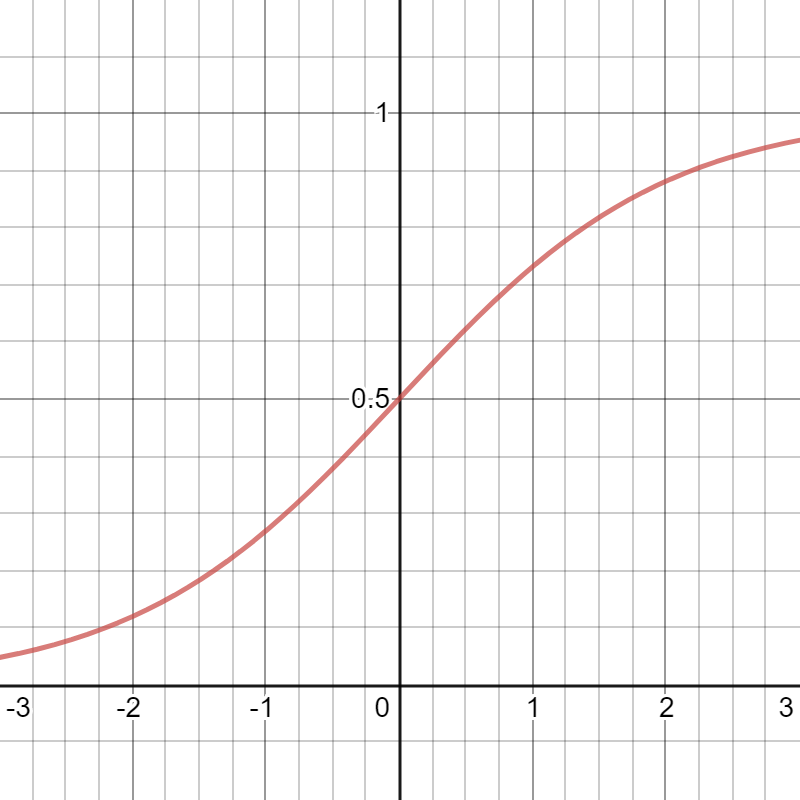
\includegraphics[width=0.9\linewidth]{activation_function_1.png}
  \caption{Sigmoid}
  \label{subfig:activation_function_1}
\end{subfigure}%
\begin{subfigure}{.32\textwidth}
  \centering
  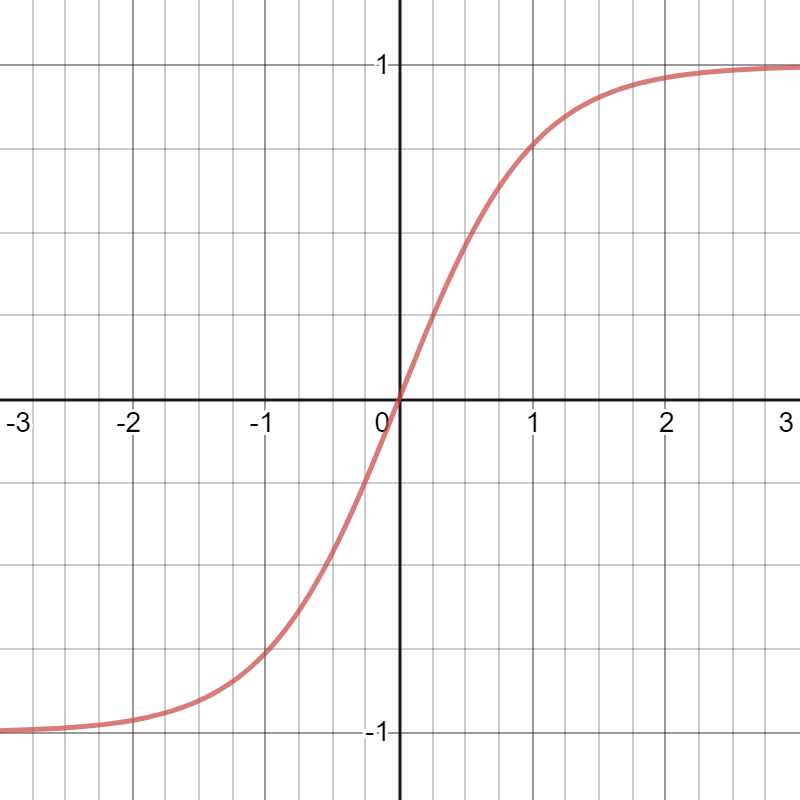
\includegraphics[width=0.9\linewidth]{activation_function_2.png}
  \caption{Tanh}
  \label{subfig:activation_function_2}
\end{subfigure}
\vskip\baselineskip
\begin{subfigure}{.32\textwidth}
  \centering
  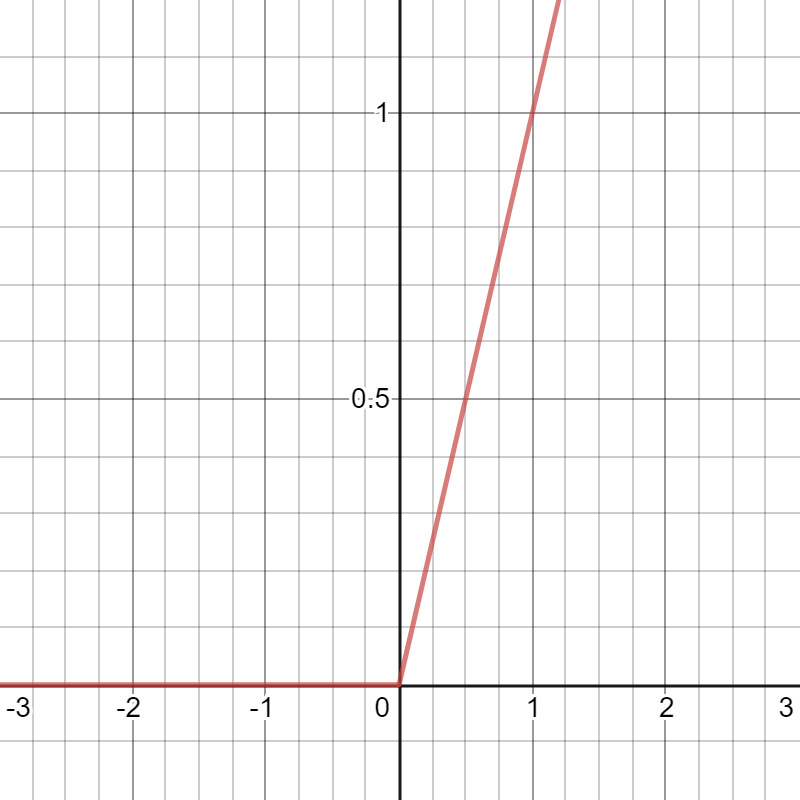
\includegraphics[width=0.9\linewidth]{activation_function_3.png}
  \caption{ReLU}
  \label{subfig:activation_function_3}
\end{subfigure}%
\begin{subfigure}{.32\textwidth}
  \centering
  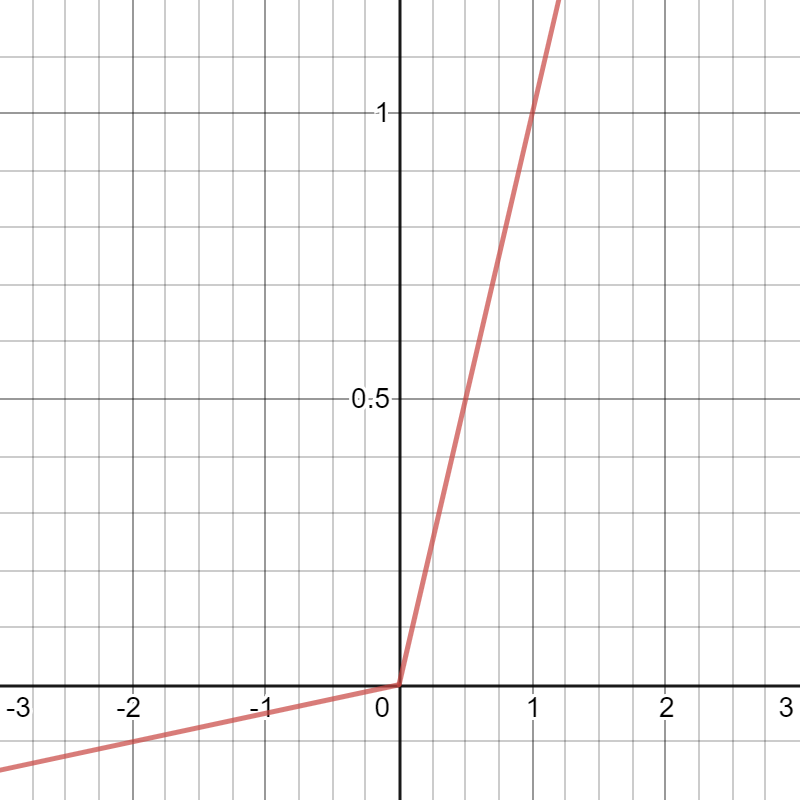
\includegraphics[width=0.9\linewidth]{activation_function_4.png}
  \caption{LeakyReLU}
  \label{subfig:activation_function_4}
\end{subfigure}
\caption{Applied activation functions}
\label{fig:activation_functions}
\end{figure}

\section{Autoencoder}

\begin{figure}[H]
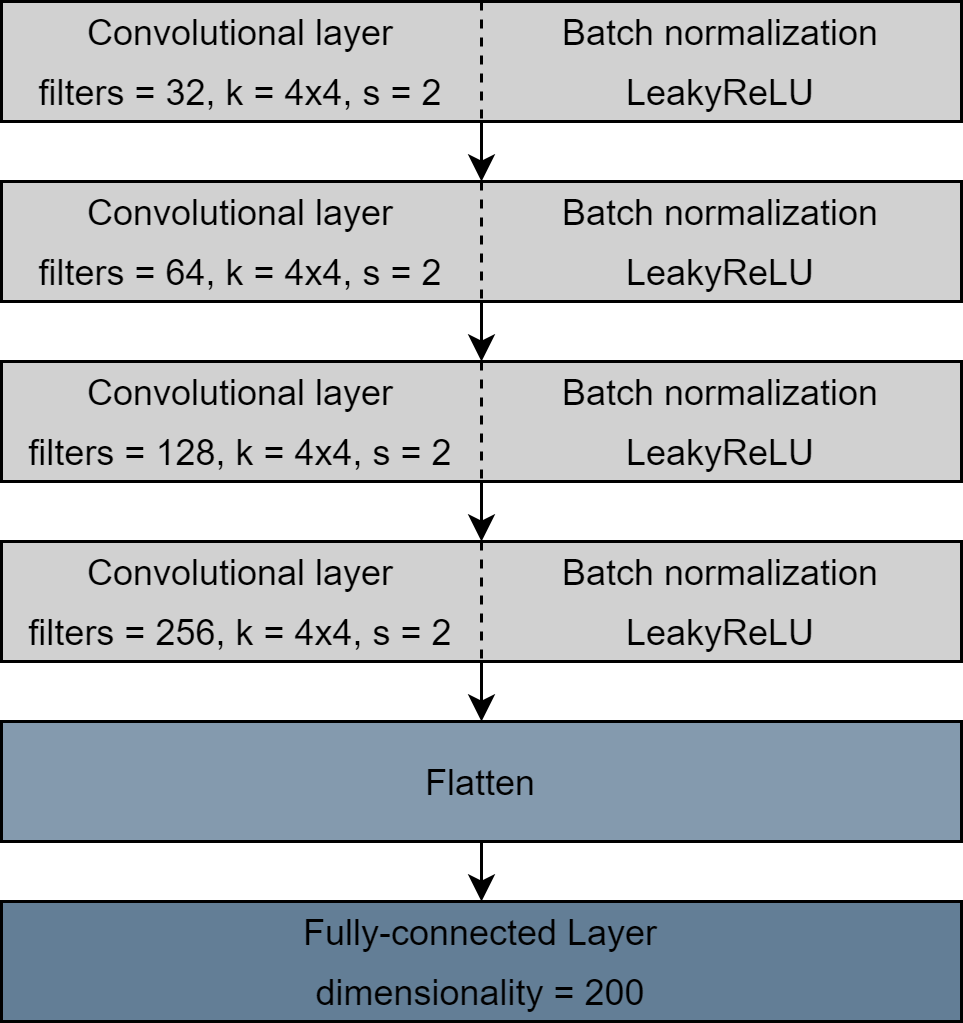
\includegraphics[width=10cm] {Models/ae_encoder.png}
\centering
\caption{Encoder architecture}
\label{fig:ae_encoder}
\end{figure}

\begin{figure}[H]
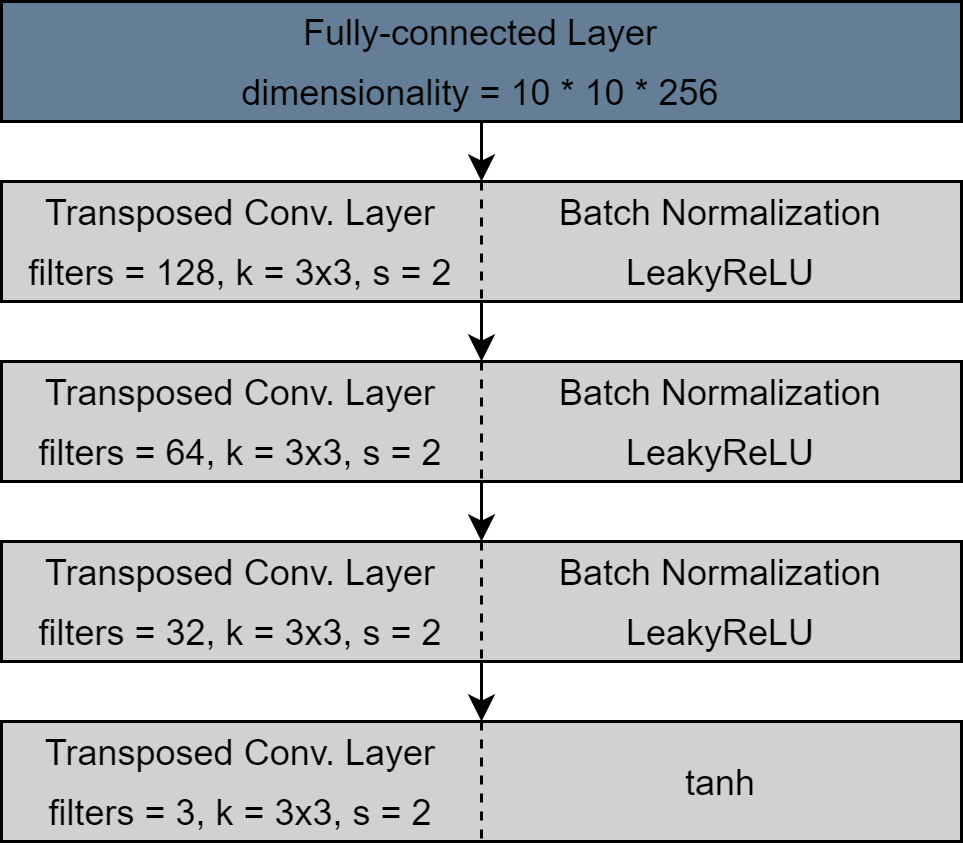
\includegraphics[width=10cm] {Models/ae_decoder.png}
\centering
\caption{Decoder architecture}
\label{fig:ae_decoder}
\end{figure}

\section{Variational autoencoder}

\begin{figure}[H]
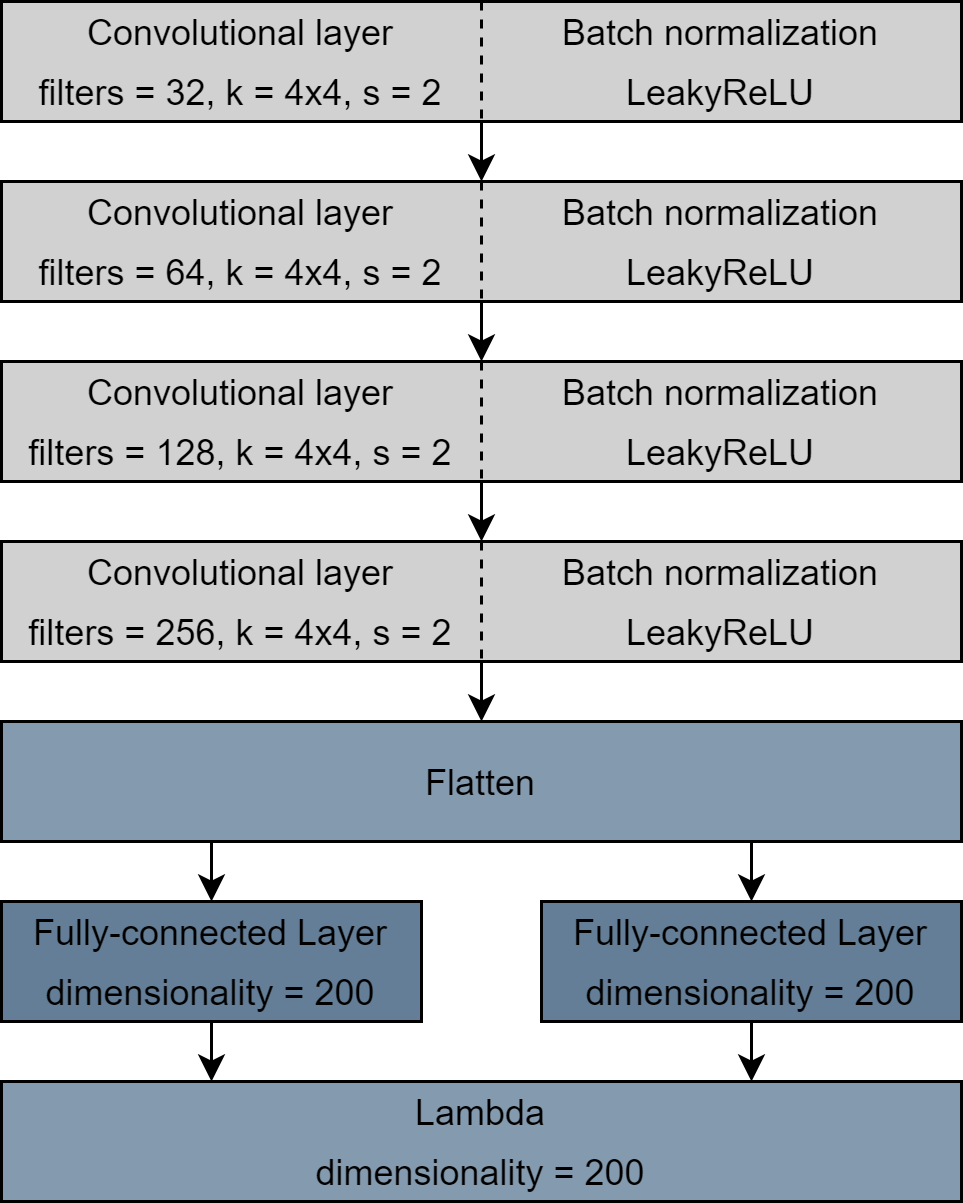
\includegraphics[width=10cm] {Models/vae_encoder.png}
\centering
\caption{Encoder architecture}
\label{fig:vae_encoder}
\end{figure}

\begin{figure}[H]
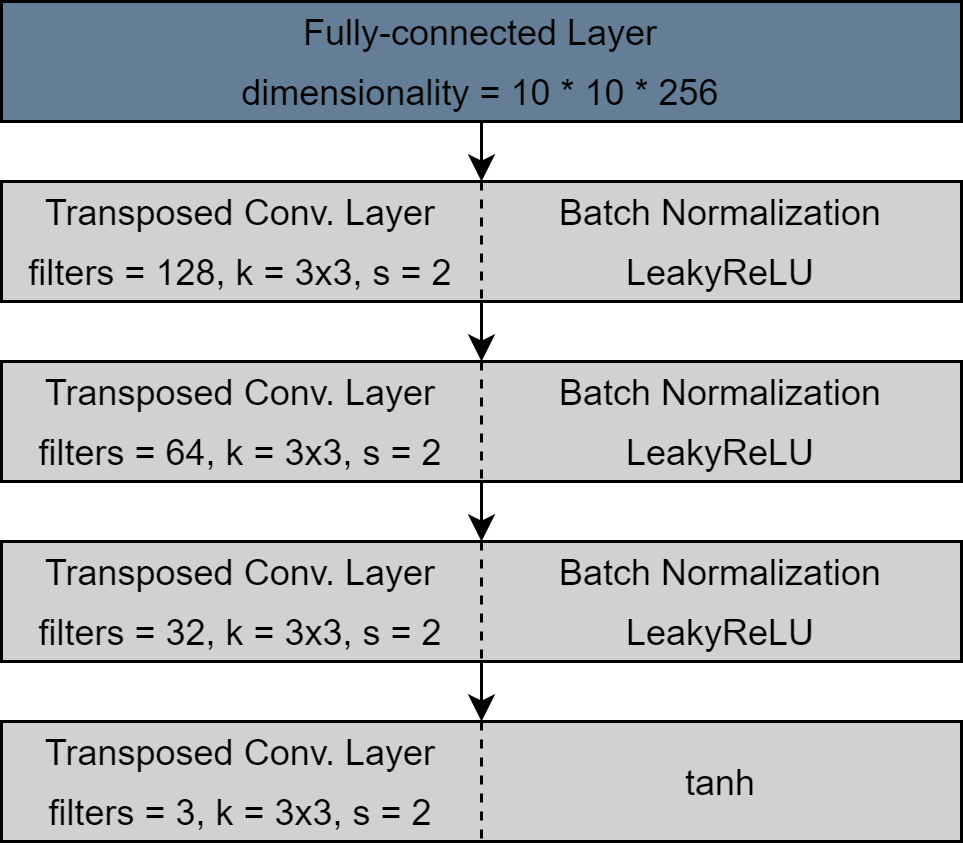
\includegraphics[width=10cm] {Models/vae_decoder.png}
\centering
\caption{Decoder architecture}
\label{fig:vae_decoder}
\end{figure}

\section{VAE-GAN}

\begin{figure}[H]
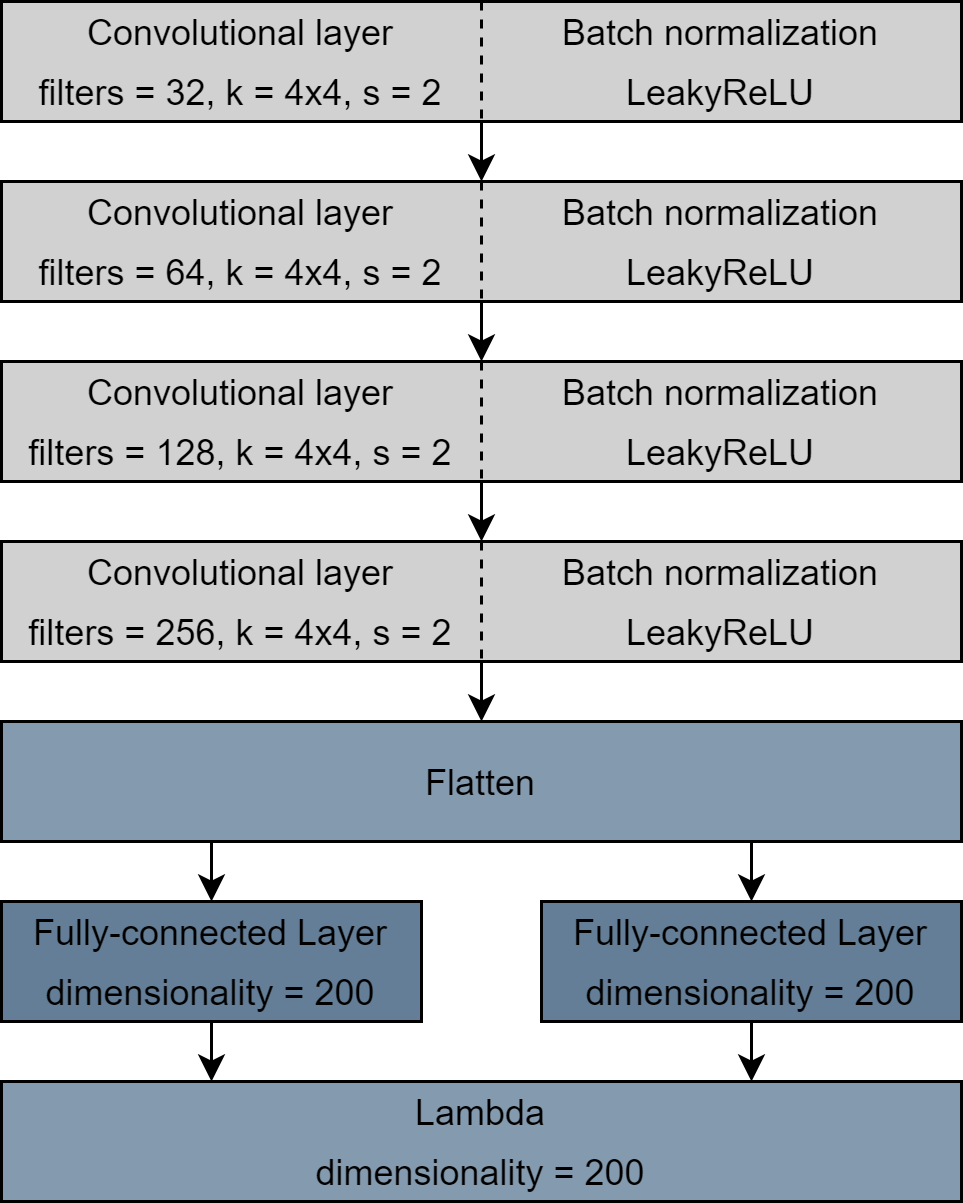
\includegraphics[width=10cm] {Models/vaegan_encoder.png}
\centering
\caption{Encoder architecture}
\label{fig:vaegan_encoder}
\end{figure}

\begin{figure}[H]
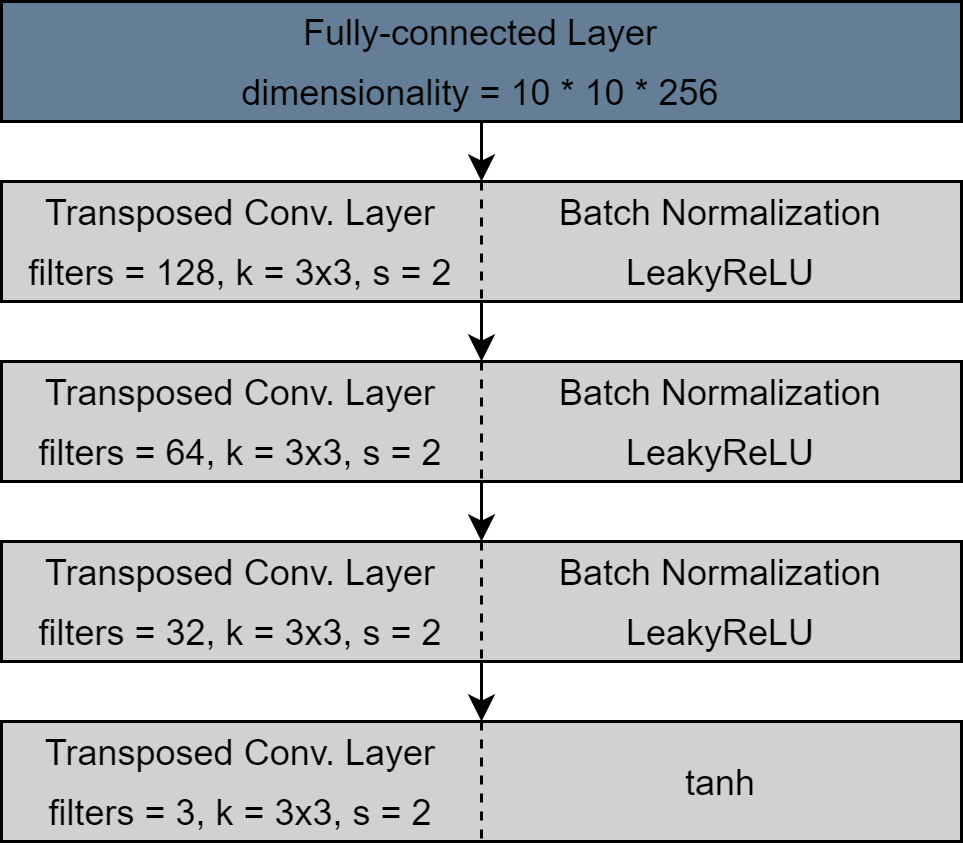
\includegraphics[width=10cm] {Models/vaegan_generator.png}
\centering
\caption{Generator architecture}
\label{fig:vaegan_generator}
\end{figure}

\begin{figure}[H]
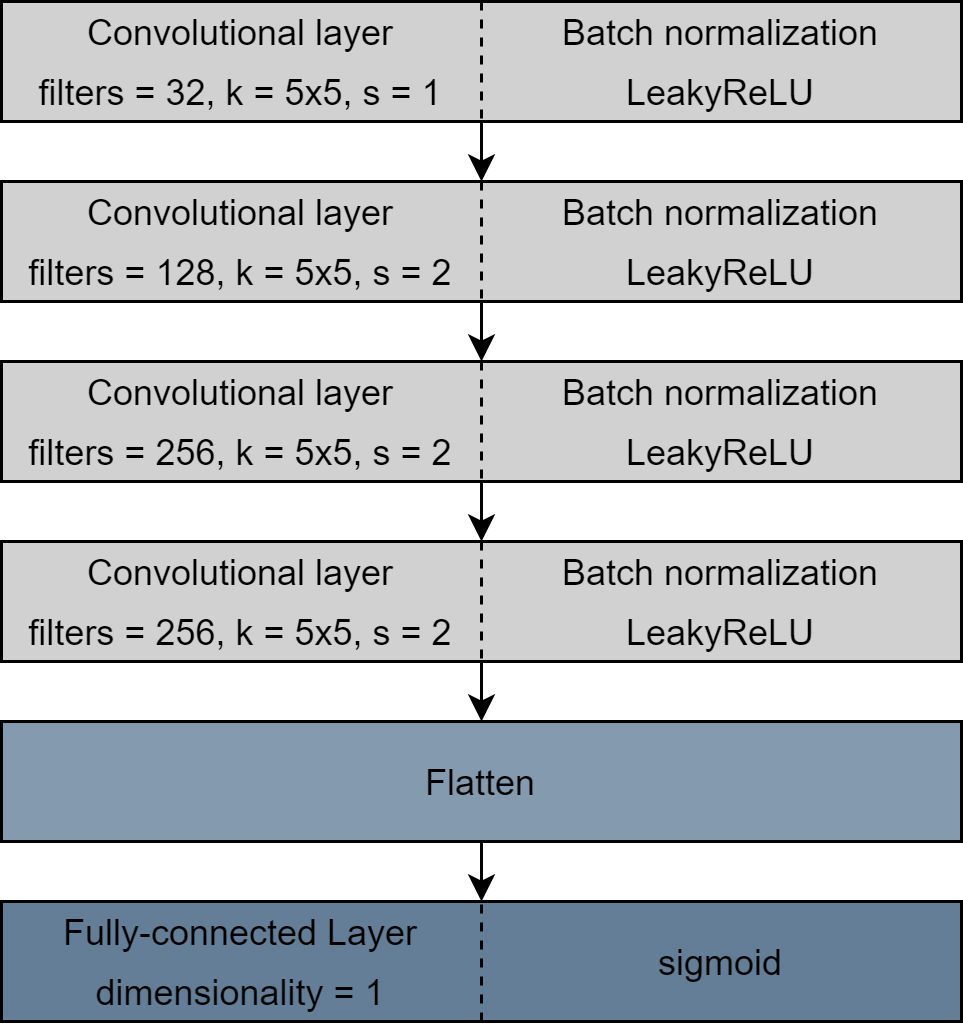
\includegraphics[width=10cm] {Models/vaegan_discriminator.png}
\centering
\caption{Discriminator architecture}
\label{fig:vaegan_dicriminator}
\end{figure}

\section{CycleGAN}

\begin{figure}[H]
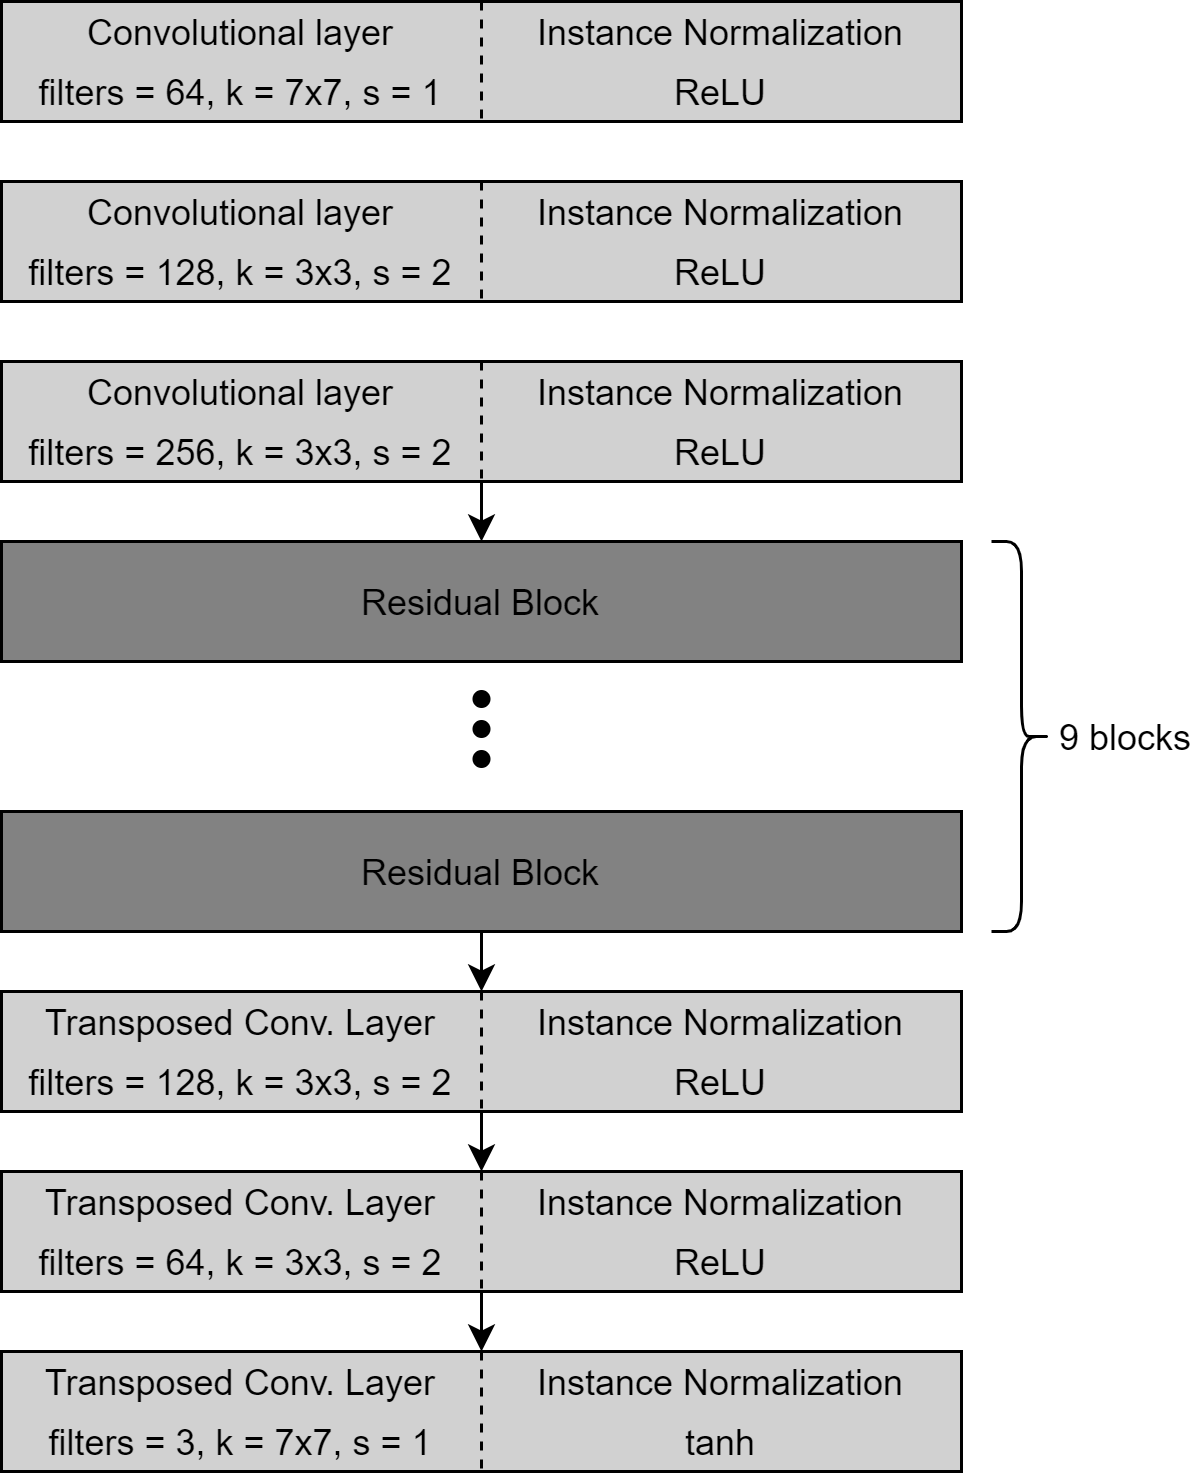
\includegraphics[width=13cm] {Models/cyclegan_generator.png}
\centering
\caption{Generator architecture}
\label{fig:cyclegan_generator}
\end{figure}

\begin{figure}[H]
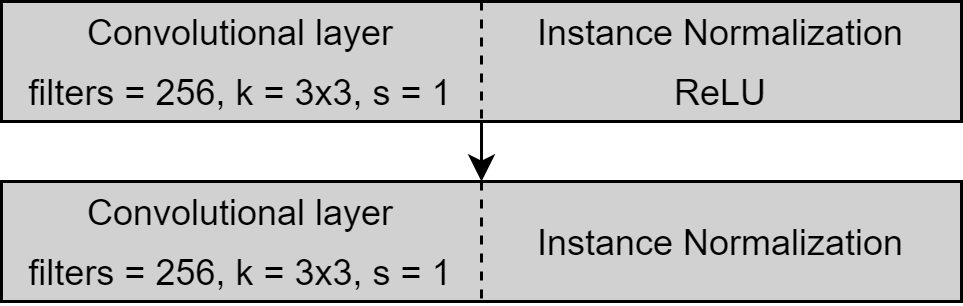
\includegraphics[width=10cm] {Models/cyclegan_residual.png}
\centering
\caption{Residual block architecture}
\label{fig:cyclegan_residual}
\end{figure}

\begin{figure}[H]
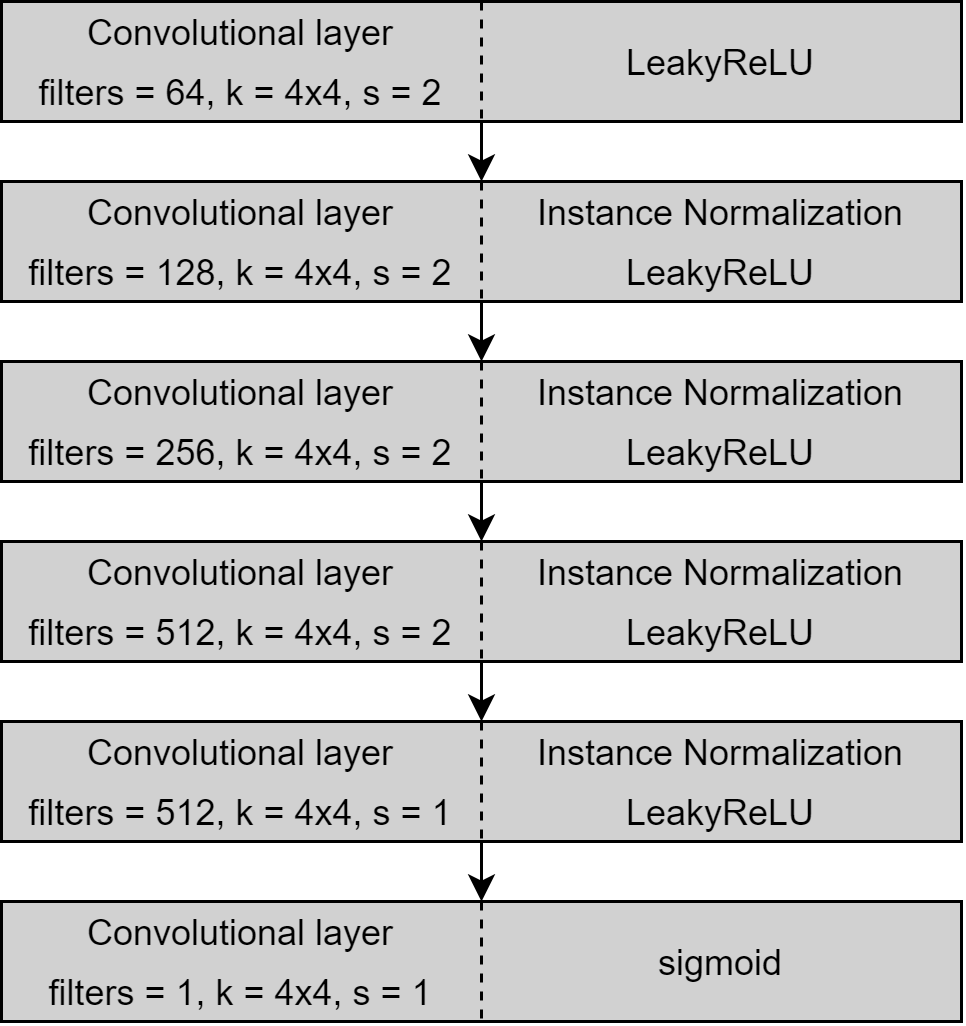
\includegraphics[width=10cm] {Models/cyclegan_discriminator.png}
\centering
\caption{Discriminator architecture}
\label{fig:cyclegan_generator}
\end{figure}
\chapter{Results}
To ensure comparability of results obtained from each implemented method, all details related to network topologies and training process, except for those that are specific for analyzed approach, should be unified. It is especially important in case of techniques which incorporate autoencoder idea, as dimensionality of latent space, may have great impact on final results, and therefore should be kept the same for each method. Such assumptions ensure that all differences in results arise from exceptional quality of particular technique.\\

Additionally, to be able to fairly evaluate effectiveness of each implemented method, for all cases, the same set of images was used to generate final results. Images come from original dataset and were selected to cover different head positions, facial expressions and lightning conditions.

\section{Autoencoder}
The encoder and decoder XY are trained as long as there is a noticeable improvement in loss function, which in this particular case was 150 epochs, as shown in figure \ref{fig:ae_decoderXY}. If the training process would be prolonged, overfitting would occur and the encoder would lose the generalization ability.

\begin{figure}[H]
\centering
\begin{subfigure}{.5\textwidth}
  \centering
  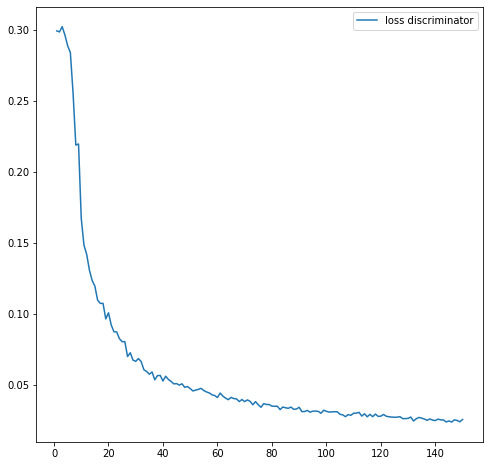
\includegraphics[width=1\linewidth]{ae_decoderXY_loss.png}
  \caption{Loss function}
  \label{subfig:ae_decoderXY_loss}
\end{subfigure}%
\begin{subfigure}{.5\textwidth}
  \centering
  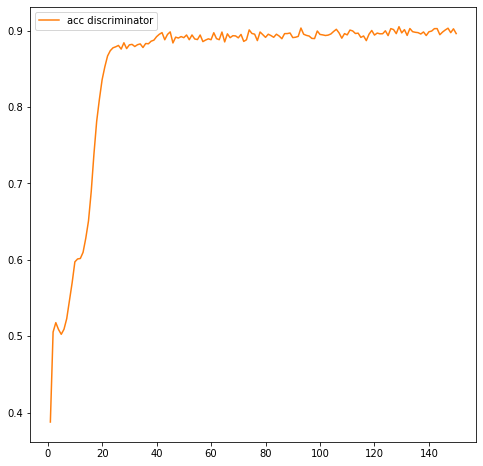
\includegraphics[width=1\linewidth]{ae_decoderXY_acc.png}
  \caption{Accuracy}
  \label{subfig:ae_decoderXY_acc}
\end{subfigure}
\caption{Training process of encoder and decoder XY}
\label{fig:ae_decoderXY}
\end{figure}

\section{Variational autoencoder}
\section{VAE-GAN}
\section{CycleGAN}
\chapter{Conclusions}
\label{Conclusions}
\section{Results analysis}
Final results of each implemented method were analyzed in terms of five main factors, which are: overall resemblance, correct head position, image sharpness, correct facial expression and lack of artifacts or deformations in the image. Correct depiction of all of those features results in obtaining high-quality deepfake. Mentioned aspects are summarized in table \ref{tab:summary_of_results}, where for each technique, presence (+) or absence (-) of each factor are marked.

\begin{table}[H]
\centering
\begin{tabular}[c]{|c|c|c|c|c|} \hline
\textbf{Feature} & \textbf{AE} & \textbf{VAE} & \textbf{VAE-GAN} & \textbf{CycleGAN}\\ \hline
Overall resemblance & + & + & + & -\\ \hline
Head position & + & + & + & +\\ \hline
Sharpness & - & - & + & +\\ \hline
Facial expression & - & - & - & +\\ \hline
Lack of artifacts/deformations & - & + & - & -\\ \hline
\end{tabular}
\caption{Summary of results}
\label{tab:summary_of_results}
\end{table}

As shown in the table above, none of the methods resulted in perfect-like deepfakes. A common feature of all techniques is correct depiction of head position, and the most problematic aspects were facial expression, and image artifacts or deformations. It is assumed that ``overall resemblance'' is the most important factor, as without it, generated images cannot be qualified as successful deepfakes, even if the rest of features is correctly depicted. This is the case of CycleGAN method, which produced the worst results in this research, despite being the only technique that correctly recreated original facial expressions.\\

Autoencoders method resulted in relatively believable deepfakes. Its shortages come from the fact that the encoder part reproduces given input by ``memorizing'' it. This characteristic, combined with dataset consisting of only two people, causes the encoder part to overfit, even in very short (epoch-wise) training. It causes the latent face to contain certain features characteristic only for original person, which cannot be later decoded by opposite-domain decoder. As a result, some artifacts or small deformations are present in the final outcome.\\

Variational autoencoders method resulted in slightly better outcomes than autoencoders technique, as it has all the advantages of AEs but do not generate images with artifacts nor deformations. This improvement arises from unique
properties of VAEs method, which produces feature maps that follow a unit Gaussian distribution. This characteristic enhance the generalization ability of the encoder part in comparison with autoencoders method.\\

In variational autoencoders generative adversarial networks method, absence of artifacts and deformations was ``sacrificed'' for the sake of better depiction of details characteristic for deepfaked person. In this cases, again, the generalization ability of the encoder network was partially lost due to the dataset property, and the fact that GAN parts of the model, in order to deceive the discriminator network, ``forced'' the encoder to produce feature maps that contain certain features characteristic only for original person.\\

CycleGAN method, in case of this research, generated the worst results. Such outcome was a surprise, as in case of horse to zebra conversion, the same technique proved to be very successful. It was concluded, and later confirmed \cite{cycleGAN_6_bib}, that CycleGAN approach is not well-suited for geometric changes and shape transformations. Such limitations make this technique useless in terms of deepfake generation, as color and texture conversion alone, are not sufficient for that purpose.

\section{Summary}
Each discussed method of deepfake generation was successfully implemented and tested according to the assumptions described in section \ref{Objective and assumptions}. None of them resulted in truly believable deepfakes, but the best outcomes were achieved in case of variational autoencoders technique. It seems that the VAE-GAN method is the one with the greatest potential, as in case of feature maps with better quality, this approach could provide deceivingly resembling fakes.\\

Main difficulty encountered in the implementation process was assessing the results obtained from each method. As there is no numerical way of measuring the quality of images obtained from deepfake algorithms, it was difficult at times, to decide if applied fine-tuning of network's parameters resulted in better or worse effects. Another encountered obstacle, was the fact, that there is no precise recipe for constructing dataset. There are a lot of factors that should be taken into a consideration when collecting data for training purposes and the complexity of this problem could be a material for a research paper on its own.\\

Further improvement of effects provided by methods based on autoencoders approach (AE, VAE, VAE-GAN) might be achieved by improving generalization ability of the encoder part. This might be done by training the encoder network on data containing images of hundreds or even thousands different people, with wide range of facial expressions. Latent faces generated  by such encoder, processed by decoders trained on targeted data might result in high-quality deepfakes, especially in case of GAN-based generators.

\bibliographystyle{ieeetran} %Sort by appearance
\bibliography{./Sections/Bibliography}

\listoffigures
\addcontentsline{toc}{chapter}{List of Figures}
\listoftables
\addcontentsline{toc}{chapter}{List of Tables}

\end{document}